%---------------------------------------------------
\chapter{MIDI support} 
\label{midi}
%---------------------------------------------------

Similarly to OSC, several \faust architectures also provide MIDI support. This allows \faust applications to be controlled from any MIDI device (or to control MIDI devices). MIDI is also the preferable way to control Polyphonic instruments.

\section{MIDI messages description in the dsp source code}

MIDI control messages are described as metadata in UI elements. They are decoded by a special architecture \emph{MidiUI} class that will parse incoming MIDI messages and update the appropriate control parameters, or send MIDI messages when the UI elements (sliders, buttons...) are moved.

\section{Description of the possible standard MIDI messages}

Below, when a 7-bit MIDI parameter is used to drive a button or
checkbox, its maximum value 127 maps to 1 ("on") while its minimum
value 0 maps to 0 ("off").

A special \lstinline'[midi:xxx yyy...]' metadata needs to be added in the UI  element description. The more usual MIDI messages can be used as described here:

- \lstinline'[midi:ctrl num]' in a slider or bargraph will map the UI element value to (0, 127) range. When used with a button or checkbox, 1 will be mapped to 127, 0 will be mapped to 0,

- \lstinline'[midi:keyon pitch]' in a slider or bargraph will register the UI element's state-variable to be driven by MIDI note-on velocity (an integer between 0 and 127) of the specified key between 0 and 127. When used with a button or checkbox, 1 will be mapped to 127, 0 will be mapped to 0,

- \lstinline'[midi:keyoff pitch]' in a slider or bargraph will register the UI element's state-variable to be driven by MIDI note-off velocity (an integer between 0 and 127) of the specified key between 0 and 127. When used with a button or checkbox, 1 will be mapped to 127, 0 will be mapped to 0,

- \lstinline'[midi:key pitch]' in a slider or bargraph will register the UI element's state-variable to be driven by MIDI note-on velocity (an integer between 0 and 127) of the specified key between 0 and 127. When used with a button or checkbox, 1 will be mapped to 127, 0 will be mapped to 0.  Note-on and note-off events will be handled,

- \lstinline'[midi:keypress pitch]' in a slider or bargraph will register the UI element's state-variable to be driven by the MIDI key-pressure (an integer between 0 and 127) from MIDI key,

- \lstinline'[midi:pgm num]' in a slider or bargraph will map the UI element value to the progchange value, so \emph{progchange} message with the same \emph{num} value will be sent. When used with a button or checkbox, 1 will send the \emph{progchange} message with \emph{num} value, 0 will send nothing,

- \lstinline'[midi:chanpress num]' in a slider or bargraph will map the UI element value to the chanpress value, so \emph{chanpress} message with the same \emph{num} value will be sent. When used with a button or checkbox, 1 will send the \emph{chanpress} message with \emph{num} value, 0 will send nothing,

- \lstinline'[midi:pitchwheel]' in a slider or bargraph will map the UI element value to (0,16383) range. When used with a button or checkbox, 1 will be mapped to 16383, 0 will be mapped to 0.

\section{A simple example}

An example with a \emph{volume} slider controlled with MIDI ctrlchange 7 messages :

\begin{lstlisting}

//-----------------------------------------------
//  Volume MIDI control in dB
//-----------------------------------------------

import("music.lib");

smooth(c) = *(1-c) : +~*(c);
gain = vslider("Volume [midi:ctrl 7]", 0, -70, +4, 0.1) : db2linear : smooth(0.999);
process = *(gain);

\end{lstlisting}

A complete testing example named  \emph{midi\_tester.dsp}  is available in the \faust distribution \emph{examples} folder.

\begin{figure}[h!]
  \centering
  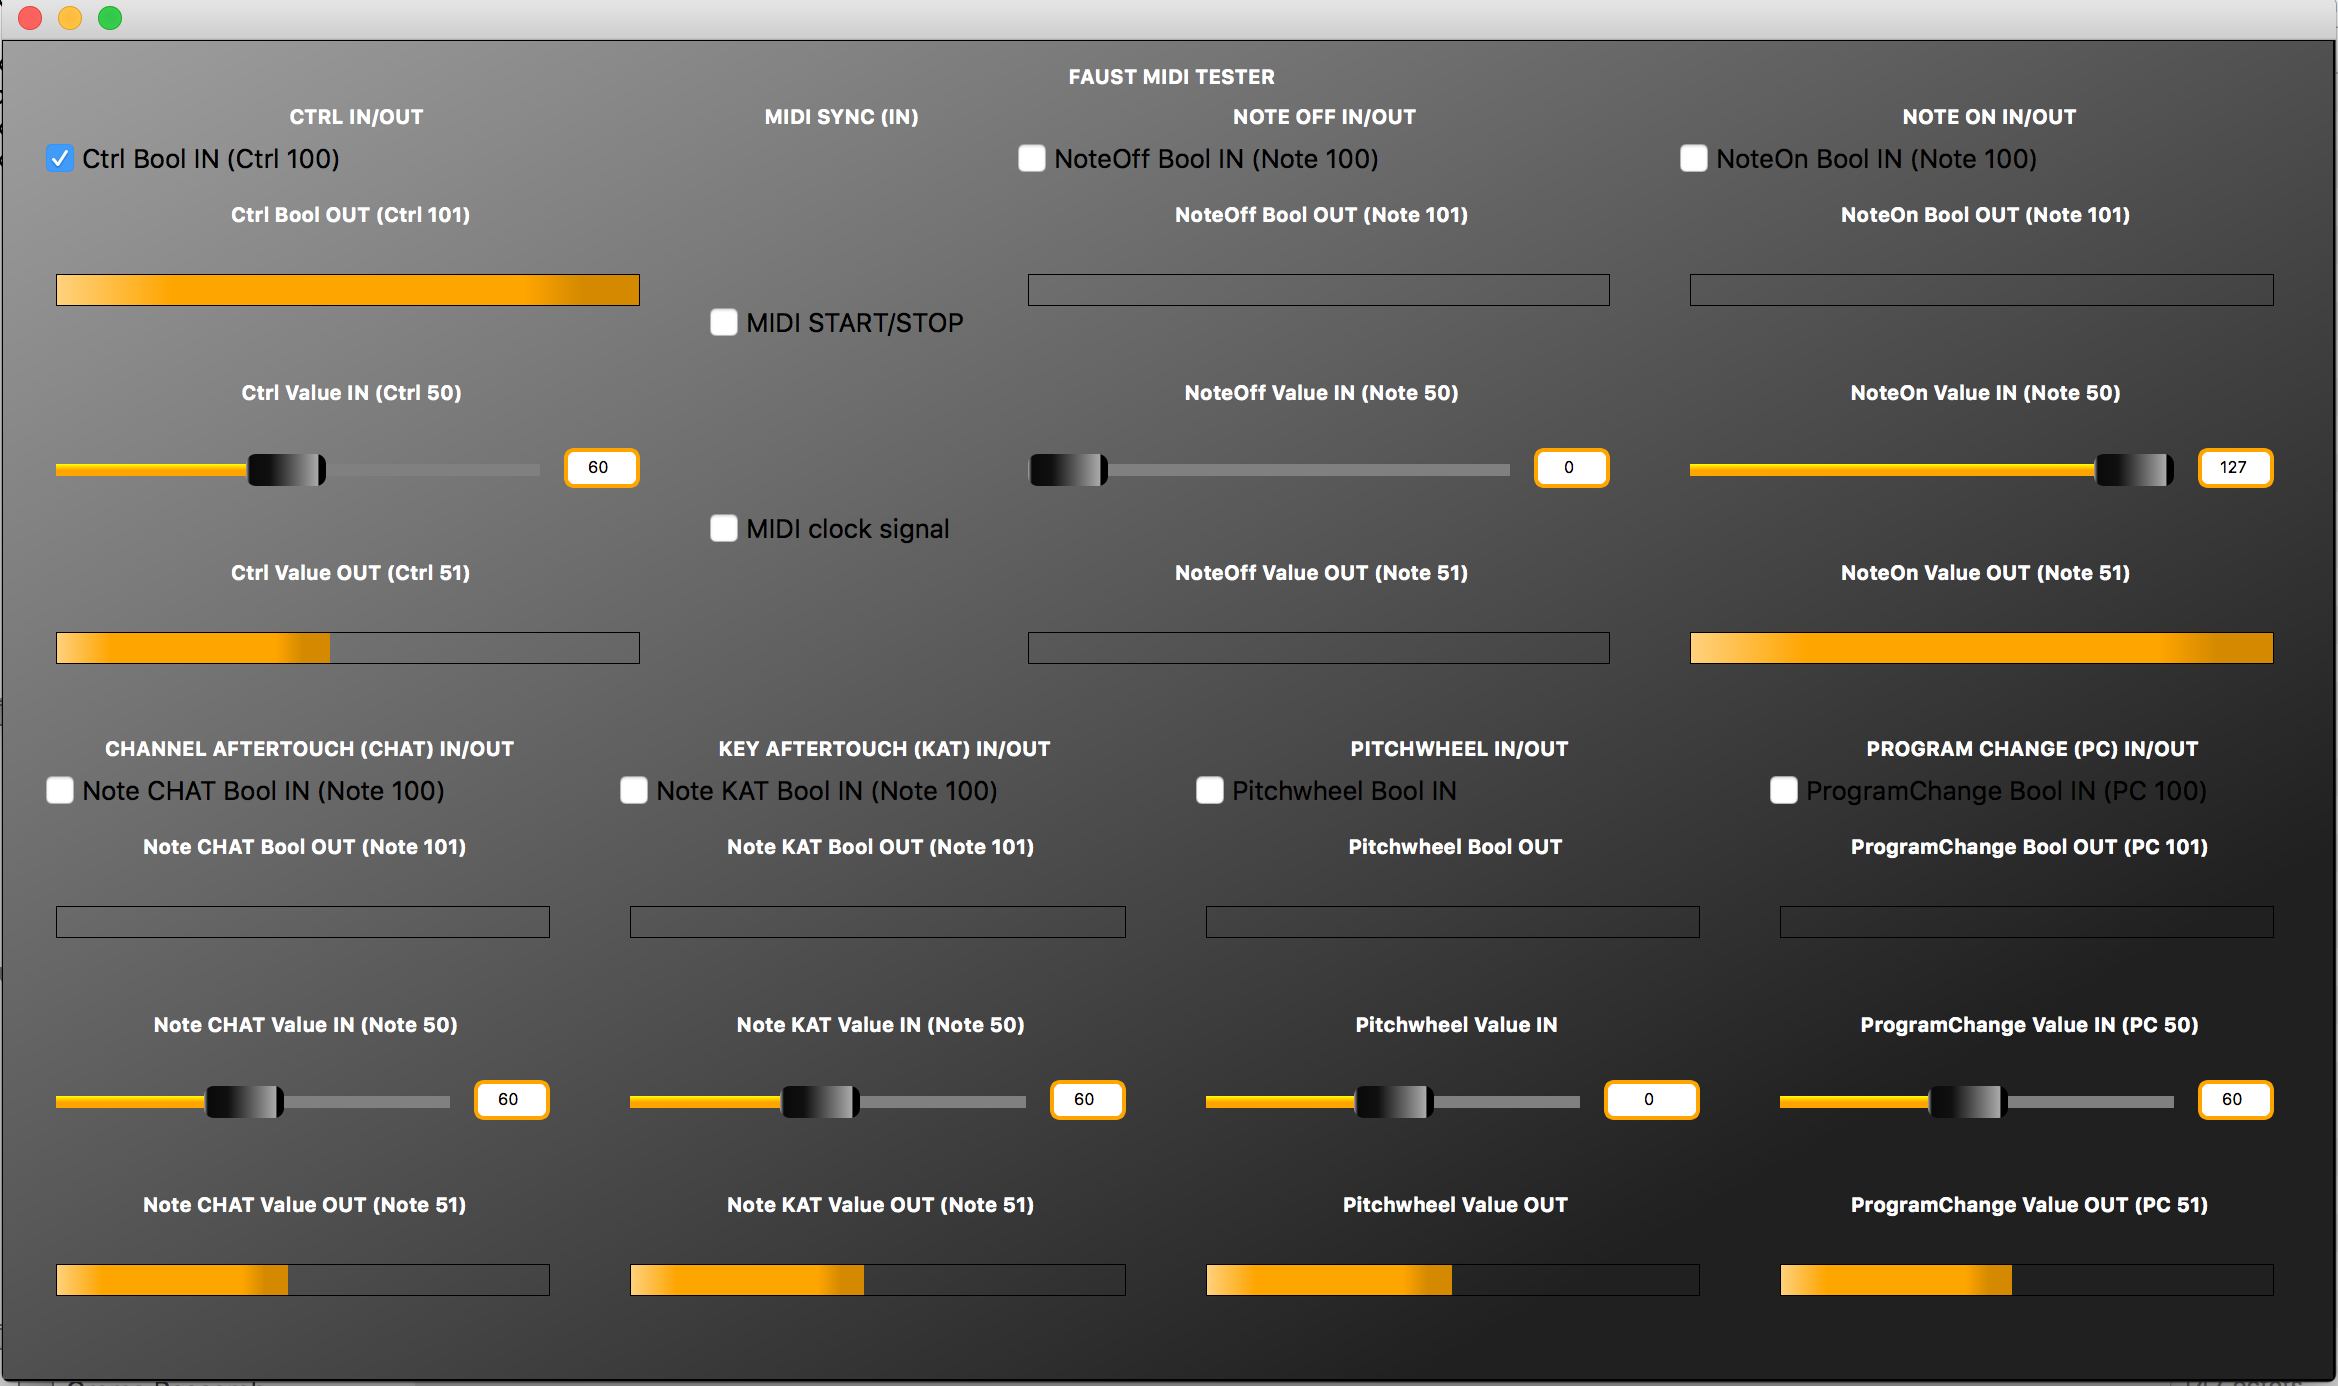
\includegraphics[width=\textwidth]{images/midi-tester.png}
  \caption{MIDI messages testing example}   
  \label{fig:midi-tester}
\end{figure}

The MIDI support can be activated using the \code{-midi} option when building the audio application with the appropriate \code{faust2xxx} command. The following table (table \ref{tab:midiarch}) lists \faust's architectures which provide MIDI support. 

\begin{table}[htp]
\begin{center}
\begin{tabular}{rcc}
\hline
\bf{Audio system} 	& \bf{Environment} & \bf{HTTP support}	\\
\hline
%\OSTab{Linux} \\
%\multicolumn{3}{|l|}{Linux} \\
%\hline
\\
\emph{Linux}\\
Alsa  		& Qt		& yes\\
Jack 			& Qt		& yes\\
%\hline
\\
\emph{Mac OS X} \\
%\hline
CoreAudio 	& Qt 	 & yes\\
Jack 			& Qt  & yes\\
%\hline
\hline
\end{tabular}
\end{center}
\caption{\faust architectures with HTTP support.}
\label{tab:midiarch}
\end{table}

\section{MIDI synchronization}

MIDI clock based synchronization can be used to slave a given Faust program. The following three messages need to be used:

- \lstinline'[midi:start]' in a button or checkbox will trigger a value of 1 when a \emph{start} MIDI message is received

- \lstinline'[midi:stop]' in a button or checkbox will trigger a value of 0 when a \emph{stop} MIDI message is received

- \lstinline'[midi:clock]' in a button or checkbox will deliver a sequence of successive 1 and 0 values each time a  \emph{clock} MIDI message is received, seen by \faust code as a square command signal, to be used to compute higher level information.

A typical Faust program will then use the MIDI clock stream to possibly compute the BPM information, or for any synchronization need it may have.  Here is a simple example of a sinus generated which a frequency controlled by the MIDI clock stream, and starting/stopping when receiving the MIDI start/stop messages:

\begin{lstlisting}
import("music.lib");

// square signal (1/0), changing state at each received clock
clocker = checkbox("MIDI clock[midi:clock]");    

// ON/OFF button controlled with MIDI start/stop messages
play = checkbox("ON/OFF [midi:start] [midi:stop]");    

// detect front
front(x) = (x-x') != 0.0;      

// count number of peaks during one second
freq(x) = (x-x@SR) : + ~ _;   
   
process = osc(8*freq(front(clocker))) * play;
\end{lstlisting}




